\documentclass[acmtog]{acmart}
\usepackage{graphicx}
\usepackage{subfigure}
\usepackage{natbib}
\usepackage{listings}
\usepackage{bm}

\definecolor{blve}{rgb}{0.3372549 , 0.61176471, 0.83921569}
\definecolor{gr33n}{rgb}{0.29019608, 0.7372549, 0.64705882}
\makeatletter
\lst@InstallKeywords k{class}{classstyle}\slshape{classstyle}{}ld
\makeatother
\lstset{language=C++,
	basicstyle=\ttfamily,
	keywordstyle=\color{blve}\ttfamily,
	stringstyle=\color{red}\ttfamily,
	commentstyle=\color{magenta}\ttfamily,
	morecomment=[l][\color{magenta}]{\#},
	classstyle = \bfseries\color{gr33n}, 
	tabsize=2
}
\lstset{basicstyle=\ttfamily}

% Title portion
\title{Assignment 3:\\ {}} 

\author{Name:\quad Xiaohan Wu  \\ student number:\ 2019533093
\\email:\quad wuxh@shanghaitech.edu.cn}

% Document starts
\begin{document}
\maketitle

\vspace*{2 ex}

\section{Introduction}
\qquad In HW3, we are required to implement the basic ray-tracing with direct illumination using the Phong lighting model. The program contains 4 basic parts and 1 optional part. The four parts are: 1.Implement a pin-hole camera model, which is able to shoot a set of optical rays. And there should be at least one ray per pixel.
2.Implement the algorithm for the ray-triangle intersection (without the acceleration structure)
3.Implement the algorithm for the ray-cube intersection based on the ray-triangle intersection (without the acceleration structure). 
4.Implement anti-aliasing for ray-tracing by using super-sampling with the rotated grid.And the optional part is to implement the texturing.
\section{Implementation Details}
\qquad In this section, I will introduce how I implement my program for each part respectively.
\\\indent 1.The realization of Pin-hole camera model is relatively easy after being given a sight from "Ray Tracing in One Weekend". I set up two vectors called "horzion" and "vertical",which are calculated from the up,forward,right of the camera and can help us transpose the coordinate of the pixel we are shooting at from screen space to world space.Thus with the position of the camera, we can easily calculate the direction of the ray and information regarding to it. 
\\\indent 2.After generating the ray where we want to shoot,we start to test ray-triangle intersection.Given the site, we adopt Moller-Trumbore intersection algorithm, where the basic idea is to find a point satisfying both the equation of ray and equation of ray and the equation of triangle. After simplfying the equation, we can get the formula listed as below.
\begin{figure}[h]
	\centering
	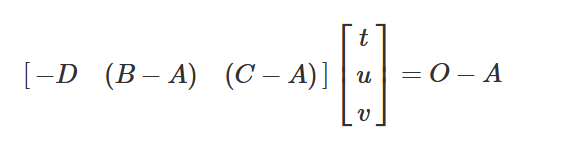
\includegraphics[width=9cm,height=2.5cm]{equation1.PNG}
	\caption{Simplified equation of Möller-Trumbore algorithm}
\end{figure}
where A,B,C means the vertices of the triangle we are going to intersect, and D is the ray vector. u,v are the  barycentric coordinate, and t is the distance from the ray's origin to the intersection .
\\\indent 3.After finishing the procedure of how to calculate the intersection of the ray and the triangle, here we are going to enable area light. For simplicity, I sample the area light uniformly in a grid pattern to form a collection of point light sources ,which are 5*5 lights in total.Also note,as there are 25samples on a uniform area light with total radiance of L, the radiance of each sample is L/25.
\\\indent 4.In order to calculate the returned radiance of the intersection point (from camera ray to scene object), we need to implement the rendering equation in the discrete case shown as below.
\begin{figure}[h]
	\centering
	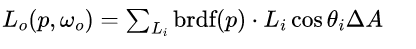
\includegraphics[width=9cm,height=1cm]{BRDF.PNG}
	\caption{Rendering equation}
\end{figure}
\\\indent However, it's relatively difficult to calculate such equation directly, aso we approximate the BRDF term by using Phong model, which we have accessed a lot. The main principle of Phong model is ommited here. And this approximation sets up the assumption that the light ray directly reach the surface of the objects, and we neglect the rays that have been reflected for multiple times.
\\\indent Following the assumption, we can then generate the ray from the light source to the intersection points. Here, the light source is just te light samples we get in the last step. And during the realization of Phong model, we have to notice the judgement of whether such ray has been blocked by other objects. If so, we have to neglect the specular and diffuse component of Phong model,only leave the ambient light. The figure below concretely exhibits the direct lighting model.
\begin{figure}[h]
	\centering
	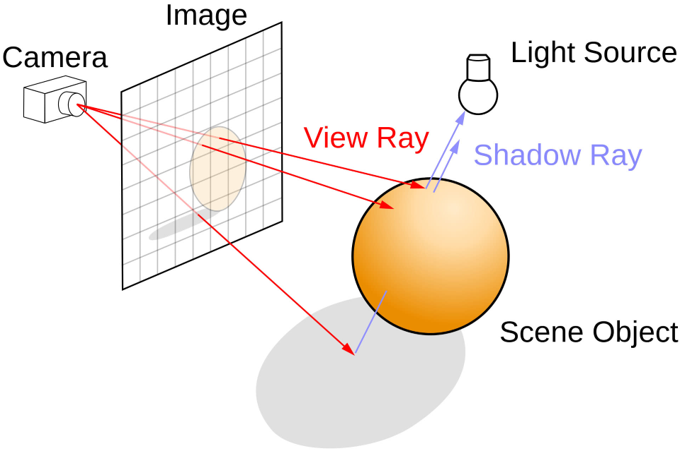
\includegraphics[width=9cm,height=5cm]{model.png}
	\caption{Phong lighting model}
\end{figure}
\\\indent 5.To avoid anti-aliasing effect, here we use the rotated grid pattern.For an optimal pattern, the rotation angle is arctan(1/2).Therefore, I use python to rotate the axis with 26.6°, sample the ones within in the range of [-0.5,0.5]*[-0.5,0.5].The sampling is shown as below. The center point denotes the center of the pixel.
\begin{figure}[h]
	\centering
	\includegraphics[width=9cm,height=6cm]{Sampling.PNG}
	\caption{Sampling display}
\end{figure}
\\\indent Therefore, we only need to note down the relative position of the samples to the center of the pixel. Each time we iterate through the pixels, we can easily calculte where we want to shoot the rays, calculate the average returned radiance to get the RGB color of the pixel.
\\\indent 6.For the texturing part, first we need to calculate the texture cooridinates (u,v) of the intersection point through interpolation. And then we map (u,v) to the pixel cooridinate to get the pixel color. Also, remember to scale the color to [0,1]*[0,1]*[0,1] to fit the vec3 color.
\section{Results}
\qquad Below are the results of my programming work.The first three ones represent results under different camera and light settings. And the last two represents the texture map and corresponding results respectively.
\begin{figure}[h]
	\centering
	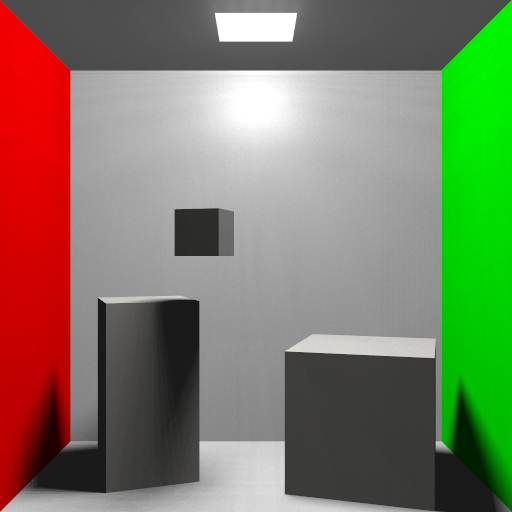
\includegraphics[width=9cm,height=9cm]{output.png}
\end{figure}
\begin{figure}[h]
	\centering
	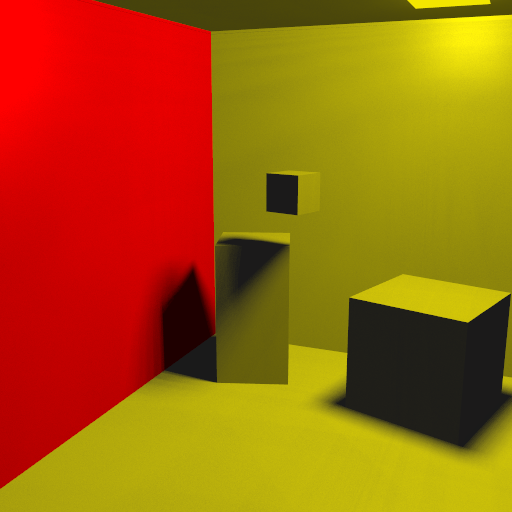
\includegraphics[width=9cm,height=9cm]{output1.png}
\end{figure}
\begin{figure}[h]
	\centering
	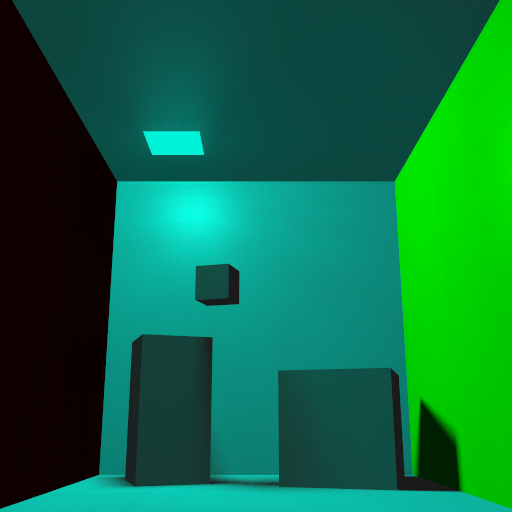
\includegraphics[width=9cm,height=9cm]{output2.png}
\end{figure}
\begin{figure}[h]
	\centering
	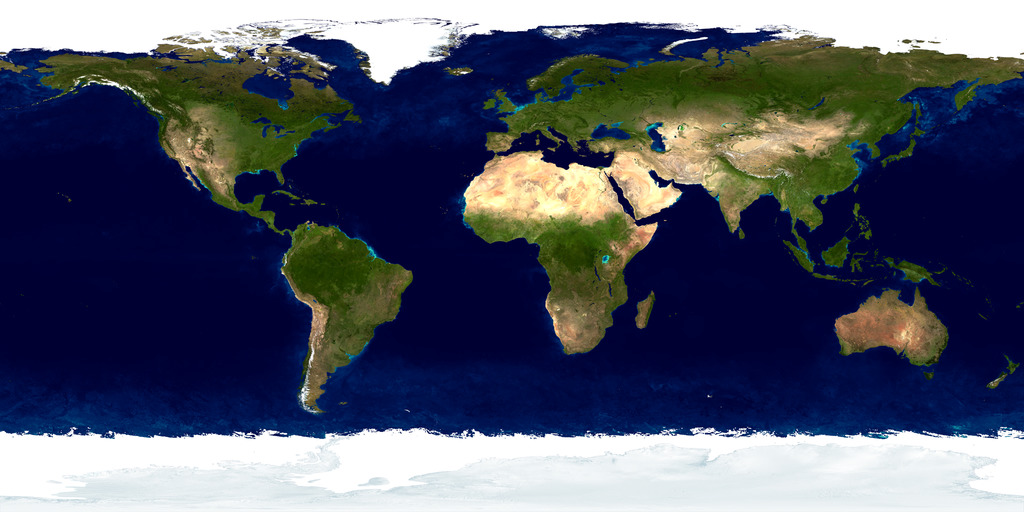
\includegraphics[width=9cm,height=5cm]{earthmap.jpg}
\end{figure}
\begin{figure}[h]
	\centering
	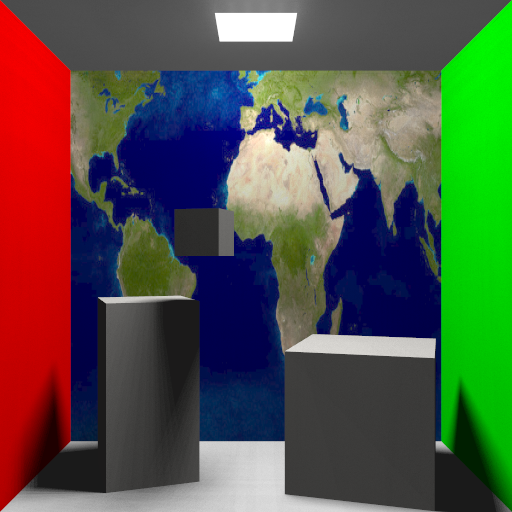
\includegraphics[width=9cm,height=9cm]{earth.png}
\end{figure}
\end{document}
